%!TeX encoding = UTF-8
%!TeX program = xelatex
\documentclass[notheorems, aspectratio=54]{beamer}
% aspectratio: 1610, 149, 54, 43(default), 32

\usepackage{latexsym}
\usepackage{amsmath,amssymb}
\usepackage{mathtools}
\usepackage{color,xcolor}
\usepackage{graphicx}
\usepackage{algorithm}
\usepackage{amsthm}
\usepackage{lmodern} % 解决 font warning
% \usepackage[UTF8]{ctex}
\usepackage{animate} % insert gif

\usepackage{lipsum} % To generate test text 
\usepackage{ulem} % 下划线,波浪线

\usepackage{listings} % display code on slides; don't forget [fragile] option after \begin{frame}

% ----------------------------------------------
% tikx
\usepackage{framed}
\usepackage{tikz}
\usepackage{pgf}
\usetikzlibrary{calc,trees,positioning,arrows,chains,shapes.geometric,%
    decorations.pathreplacing,decorations.pathmorphing,shapes,%
    matrix,shapes.symbols}
\pgfmathsetseed{1} % To have predictable results
% Define a background layer, in which the parchment shape is drawn
\pgfdeclarelayer{background}
\pgfsetlayers{background,main}

% define styles for the normal border and the torn border
\tikzset{
  normal border/.style={orange!30!black!10, decorate, 
     decoration={random steps, segment length=2.5cm, amplitude=.7mm}},
  torn border/.style={orange!30!black!5, decorate, 
     decoration={random steps, segment length=.5cm, amplitude=1.7mm}}}

% Macro to draw the shape behind the text, when it fits completly in the
% page
\def\parchmentframe#1{
\tikz{
  \node[inner sep=2em] (A) {#1};  % Draw the text of the node
  \begin{pgfonlayer}{background}  % Draw the shape behind
  \fill[normal border] 
        (A.south east) -- (A.south west) -- 
        (A.north west) -- (A.north east) -- cycle;
  \end{pgfonlayer}}}

% Macro to draw the shape, when the text will continue in next page
\def\parchmentframetop#1{
\tikz{
  \node[inner sep=2em] (A) {#1};    % Draw the text of the node
  \begin{pgfonlayer}{background}    
  \fill[normal border]              % Draw the ``complete shape'' behind
        (A.south east) -- (A.south west) -- 
        (A.north west) -- (A.north east) -- cycle;
  \fill[torn border]                % Add the torn lower border
        ($(A.south east)-(0,.2)$) -- ($(A.south west)-(0,.2)$) -- 
        ($(A.south west)+(0,.2)$) -- ($(A.south east)+(0,.2)$) -- cycle;
  \end{pgfonlayer}}}

% Macro to draw the shape, when the text continues from previous page
\def\parchmentframebottom#1{
\tikz{
  \node[inner sep=2em] (A) {#1};   % Draw the text of the node
  \begin{pgfonlayer}{background}   
  \fill[normal border]             % Draw the ``complete shape'' behind
        (A.south east) -- (A.south west) -- 
        (A.north west) -- (A.north east) -- cycle;
  \fill[torn border]               % Add the torn upper border
        ($(A.north east)-(0,.2)$) -- ($(A.north west)-(0,.2)$) -- 
        ($(A.north west)+(0,.2)$) -- ($(A.north east)+(0,.2)$) -- cycle;
  \end{pgfonlayer}}}

% Macro to draw the shape, when both the text continues from previous page
% and it will continue in next page
\def\parchmentframemiddle#1{
\tikz{
  \node[inner sep=2em] (A) {#1};   % Draw the text of the node
  \begin{pgfonlayer}{background}   
  \fill[normal border]             % Draw the ``complete shape'' behind
        (A.south east) -- (A.south west) -- 
        (A.north west) -- (A.north east) -- cycle;
  \fill[torn border]               % Add the torn lower border
        ($(A.south east)-(0,.2)$) -- ($(A.south west)-(0,.2)$) -- 
        ($(A.south west)+(0,.2)$) -- ($(A.south east)+(0,.2)$) -- cycle;
  \fill[torn border]               % Add the torn upper border
        ($(A.north east)-(0,.2)$) -- ($(A.north west)-(0,.2)$) -- 
        ($(A.north west)+(0,.2)$) -- ($(A.north east)+(0,.2)$) -- cycle;
  \end{pgfonlayer}}}

% Define the environment which puts the frame
% In this case, the environment also accepts an argument with an optional
% title (which defaults to ``Example'', which is typeset in a box overlaid
% on the top border
\newenvironment{parchment}[1][Example]{%
  \def\FrameCommand{\parchmentframe}%
  \def\FirstFrameCommand{\parchmentframetop}%
  \def\LastFrameCommand{\parchmentframebottom}%
  \def\MidFrameCommand{\parchmentframemiddle}%
  \vskip\baselineskip
  \MakeFramed {\FrameRestore}
  \noindent\tikz\node[inner sep=1ex, draw=black!20,fill=white, 
          anchor=west, overlay] at (0em, 2em) {\sffamily#1};\par}%
{\endMakeFramed}

% ----------------------------------------------

\mode<presentation>{
    \usetheme{CambridgeUS}
    % Boadilla CambridgeUS
    % default Antibes Berlin Copenhagen
    % Madrid Montpelier Ilmenau Malmoe
    % Berkeley Singapore Warsaw
    \usecolortheme{beaver}
    % beetle, beaver, orchid, whale, dolphin
    \useoutertheme{infolines}
    % infolines miniframes shadow sidebar smoothbars smoothtree split tree
    \useinnertheme{circles}
    % circles, rectanges, rounded, inmargin
}
% 设置 block 颜色
\setbeamercolor{block title}{bg=red!30,fg=white}

\newcommand{\reditem}[1]{\setbeamercolor{item}{fg=red}\item #1}

% 缩放公式大小
\newcommand*{\Scale}[2][4]{\scalebox{#1}{\ensuremath{#2}}}

% 解决 font warning
\renewcommand\textbullet{\ensuremath{\bullet}}

% ---------------------------------------------------------------------
% flow chart
\tikzset{
    >=stealth',
    punktchain/.style={
        rectangle, 
        rounded corners, 
        % fill=black!10,
        draw=white, very thick,
        text width=6em,
        minimum height=2em, 
        text centered, 
        on chain
    },
    largepunktchain/.style={
        rectangle,
        rounded corners,
        draw=white, very thick,
        text width=10em,
        minimum height=2em,
        on chain
    },
    line/.style={draw, thick, <-},
    element/.style={
        tape,
        top color=white,
        bottom color=blue!50!black!60!,
        minimum width=6em,
        draw=blue!40!black!90, very thick,
        text width=6em, 
        minimum height=2em, 
        text centered, 
        on chain
    },
    every join/.style={->, thick,shorten >=1pt},
    decoration={brace},
    tuborg/.style={decorate},
    tubnode/.style={midway, right=2pt},
    font={\fontsize{10pt}{12}\selectfont},
}
% ---------------------------------------------------------------------

% code setting
\lstset{
    language=C++,
    basicstyle=\ttfamily\footnotesize,
    keywordstyle=\color{red},
    breaklines=true,
    xleftmargin=2em,
    numbers=left,
    numberstyle=\color[RGB]{222,155,81},
    frame=leftline,
    tabsize=4,
    breakatwhitespace=false,
    showspaces=false,               
    showstringspaces=false,
    showtabs=false,
    morekeywords={Str, Num, List},
}

% ---------------------------------------------------------------------

%% preamble
\title[Recent Paper Reading]{Resent Paper Reading}
% \subtitle{The subtitle}
\author{Fengyuan Dai}
\institute[Westlake University]{daifengyuan@westlake.edu.cn}

% -------------------------------------------------------------

\begin{document}

%% title frame
\begin{frame}
    \titlepage
\end{frame}

%% normal frame


\section{ICLR23 Paper1}
\begin{frame}
    \frametitle{Table of Contents}
    \tableofcontents[currentsection]
\end{frame}

\begin{frame}{Protein Representation Learning via Knowledge Enhanced Primary Structure Modeling}
  \begin{figure}[!h]
    \centering
    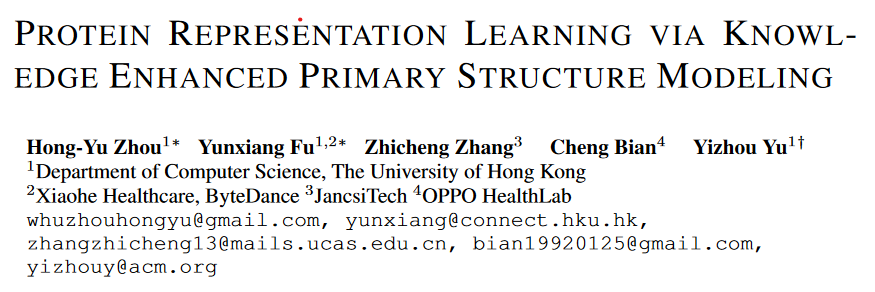
\includegraphics[width=0.9\linewidth]{figures/PRL-title.png}
  \end{figure}
  \textbf{What's new}
  \begin{itemize}
    \item Propose Knowledge-exploited Auto-encoder for Protein (KeAP). 
    \item Auto-encoder pretraining and fine-tuning on 9 representative downstream tasks.  
  \end{itemize}
\end{frame}


\begin{frame}{Protein Representation Learning via Knowledge Enhanced Primary Structure Modeling}
  \textbf{Motivations}
  \begin{itemize}
      \item Pre-trained protein models also suffer from a problem in language models: a lack of factual knowledge.
      \item Explore the relationships at a more granular level, i.e., the token level.
  \end{itemize}

  % \begin{figure}[!h]
  %   \centering
  %   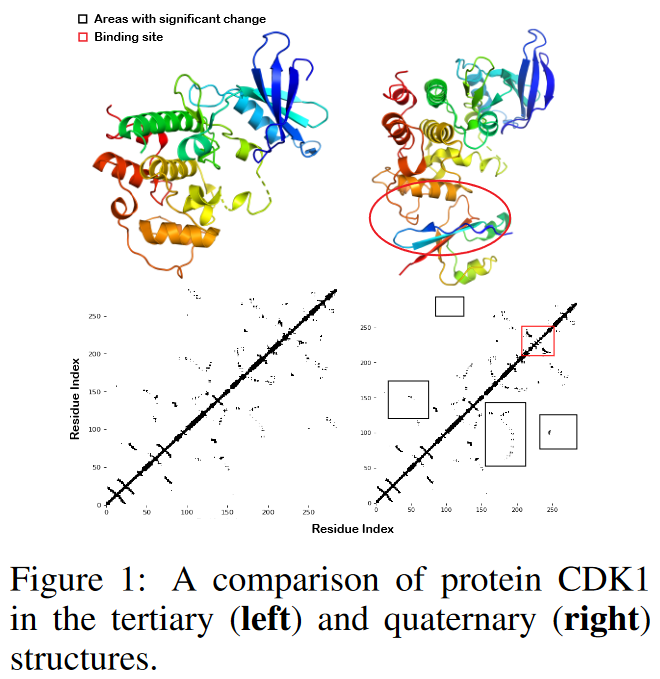
\includegraphics[width=0.4\linewidth]{figures/MPH-fig1.png}
  % \end{figure}

\end{frame}

\begin{frame}{Protein Representation Learning via Knowledge Enhanced Primary Structure Modeling}
  \textbf{Method}
  \begin{itemize}
      \item Auto-encoder architecture and masked language modeling (MLM) objective.
      \item Explore the relationships at a more granular level, i.e., the token level.
  \end{itemize}

  \begin{figure}[!h]
    \centering
    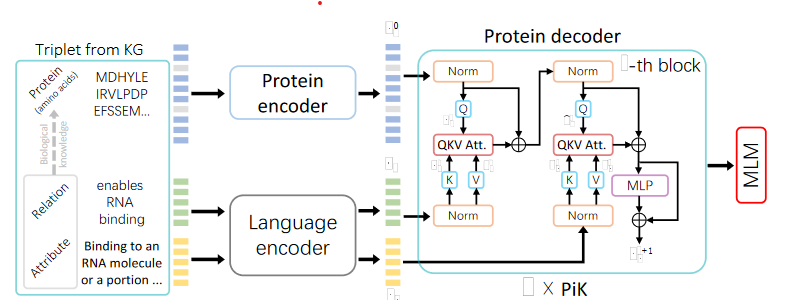
\includegraphics[width=1\linewidth]{figures/PRL-fig2.png}
  \end{figure}
\end{frame}


\begin{frame}{Protein Representation Learning via Knowledge Enhanced Primary Structure Modeling}
  \textbf{Experiments}
  \begin{itemize}
      \item Pretraining dataset: ProteinKG25.
      \item Downstream tasks: amino acid contact prediction, protein homology detection, protein stability prediction, protein interaction identification, protein-protein binding affinity prediction, and semantic similarity inference.
  \end{itemize}
  % \begin{figure}[!h]
  %   \centering
  %   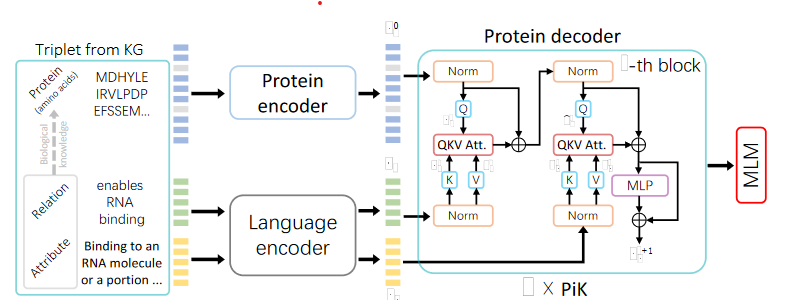
\includegraphics[width=1\linewidth]{figures/PRL-fig2.png}
  % \end{figure}
\end{frame}


\begin{frame}{Protein Representation Learning via Knowledge Enhanced Primary Structure Modeling}
  \textbf{Experiments}
  \begin{itemize}
      \item amino acid contact prediction
  \end{itemize}
  \begin{figure}[!h]
    \centering
    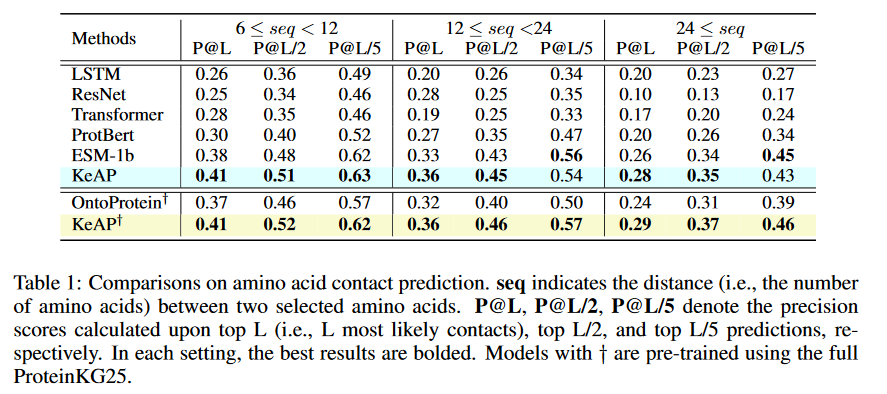
\includegraphics[width=1\linewidth]{figures/PRL-tab1.png}
  \end{figure}
\end{frame}


\section{ICLR23 Paper2}
\begin{frame}
    \frametitle{Table of Contents}
    \tableofcontents[currentsection]
\end{frame}

\begin{frame}{Multi-level Protein Structure Pre-training via Prompt Learning}
  \begin{figure}[!h]
    \centering
    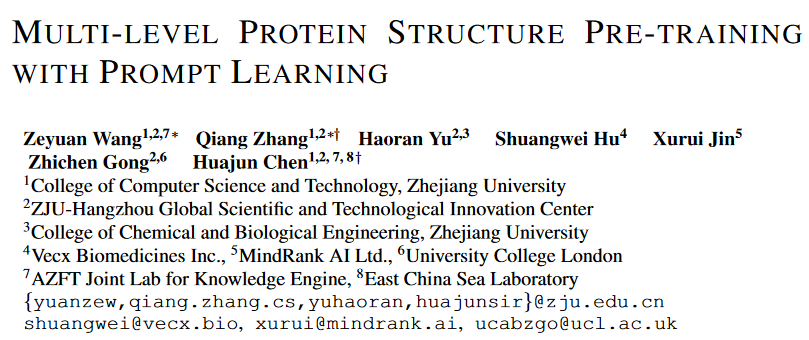
\includegraphics[width=0.85\linewidth]{figures/MPH-title.png}
  \end{figure}
  \textbf{What's new}
  \begin{itemize}
    \item Propose a new prompt-guided multi-task pretraining and fine-tuning framework.
    \item Three pretrain tasks and fine-tuning on two downstream tasks.  
  \end{itemize}

\end{frame}


\begin{frame}{Multi-level Protein Structure Pre-training via Prompt Learning}
  \textbf{Motivations}
  \begin{itemize}
      \item Most existing function prediction methods take either the primary or the tertiary structure as input, unintentionally ignoring the other levels of protein structures.
  \end{itemize}

  \begin{figure}[!h]
    \centering
    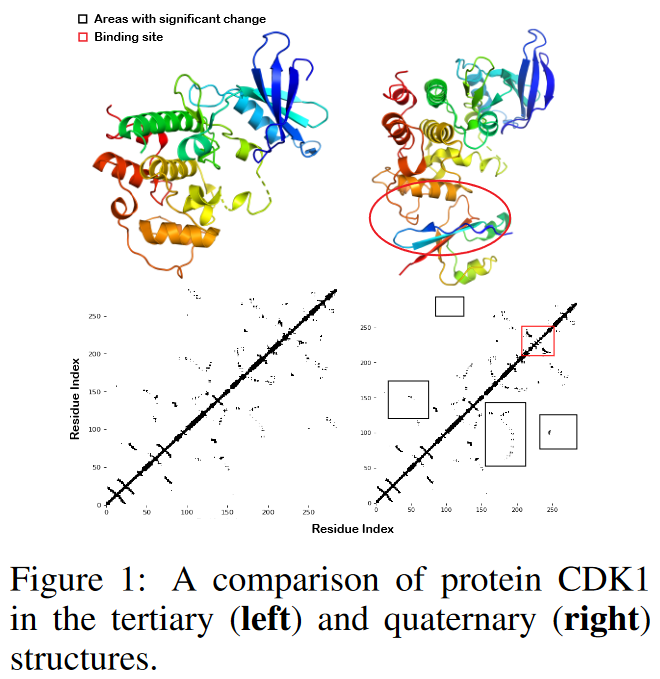
\includegraphics[width=0.4\linewidth]{figures/MPH-fig1.png}
  \end{figure}
\end{frame}


\begin{frame}{Multi-level Protein Structure Pre-training via Prompt Learning}
  \textbf{Method}
  \begin{itemize}
      \item Prompt-Aware Transformer
      \begin{itemize}
        \item Attention mask
        \item Skip connection
      \end{itemize}
  \end{itemize}

  \begin{figure}[!h]
    \centering
    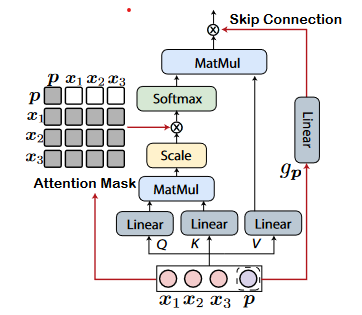
\includegraphics[width=0.5\linewidth]{figures/MPH-fig3.png}
  \end{figure}
\end{frame}

% \end{document}


\begin{frame}{Multi-level Protein Structure Pre-training via Prompt Learning}
  \textbf{Method}
  \begin{itemize}
      \item Prompt-Aware Transformer
      \begin{itemize}
        \item Attention mask
        \item Skip connection
      \end{itemize}
  \end{itemize}

  \begin{figure}[!h]
    \centering
    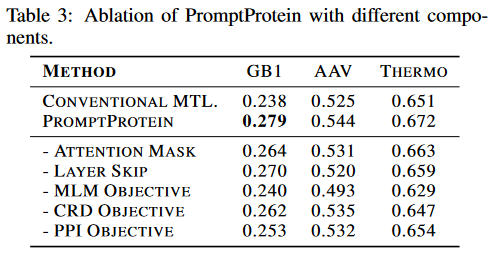
\includegraphics[width=0.6\linewidth]{figures/MPH-tab3.png}
  \end{figure}
\end{frame}

\begin{frame}{Multi-level Protein Structure Pre-training via Prompt Learning}
  \textbf{Pretraining} and Fine-tuning
  
  \begin{figure}[!h]
    \centering
    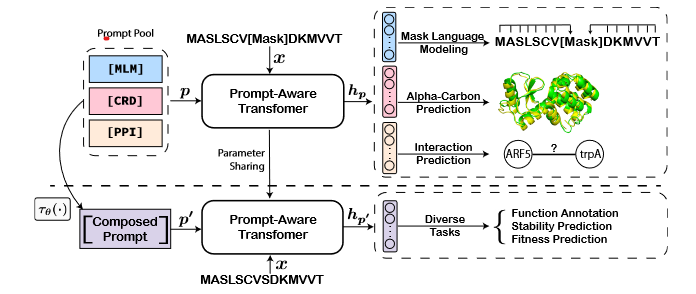
\includegraphics[width=0.9\linewidth]{figures/MPH-fig2.png}
  \end{figure}

  \begin{itemize}
    \item Masked language modeling for sequence.
    \item Alpha-carbon coordinate prediction for secondary and tertiary structures.
    \item Protein-protein interaction prediction for quaternary structure. 
  \end{itemize}
\end{frame}

% \begin{frame}{Multi-level Protein Structure Pre-training via Prompt Learning}
%   \textbf{Pretraining} and Fine-tuning
  
%   \begin{figure}[!h]
%     \centering
%     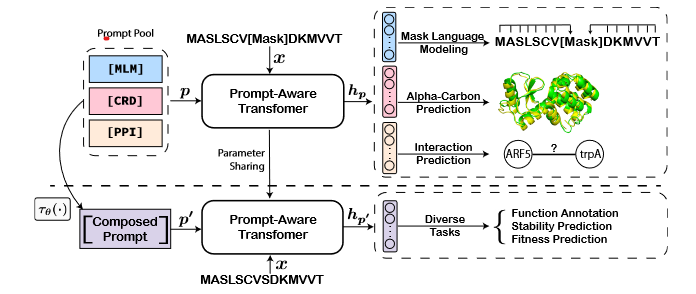
\includegraphics[width=0.9\linewidth]{figures/MPH-fig2.png}
%   \end{figure}

%   \begin{itemize}
%     \item Masked language modeling for sequence.
%     \item Alpha-carbon coordinate prediction for secondary and tertiary structures.
%     \item Protein-protein interaction prediction for quaternary structure. 
%   \end{itemize}
% \end{frame}


% \begin{frame}{Multi-level Protein Structure Pre-training via Prompt Learning}
%   \textbf{Pretraining} and Fine-tuning
  
%   \begin{itemize}
%     \item Masked language modeling for sequence.
%     \begin{itemize}
%       \item $L_{MLM}(h_p) = \sum_{y \in Y} -logq(y|h_p)$
%     \end{itemize}
%     \item Alpha-carbon coordinate prediction for secondary and tertiary structures.
%     \begin{itemize}
%       \item $L_{CRD}(h_p) = MSE(Z, Kabsh(MLP(h_p)))$
%     \end{itemize}
%     \item Protein-protein interaction prediction for quaternary structure. 
%     \begin{itemize}
%       \item $L_{PPI}(h_p) = \sum_{m,n \in N} BCE(y_{m,n}, p(y_{m,n})|h_p^{m,n})$
%     \end{itemize}
%   \end{itemize}
% \end{frame}

\begin{frame}{Multi-level Protein Structure Pre-training via Prompt Learning}
  \textbf{Pretraining} and Fine-tuning
    
    \begin{itemize}
      \item Masked language modeling for sequence.
      \begin{itemize}
        \item $$L_{MLM}(h_p) = \sum_{y \in Y} -logq(y|h_p)$$
      \end{itemize}
      \item Alpha-carbon coordinate prediction for secondary and tertiary structures.
      \begin{itemize}
        \item $$L_{CRD}(h_p) = MSE(Z, Kabsh(MLP(h_p)))$$
      \end{itemize}
      \item Protein-protein interaction prediction for quaternary structure. 
      \begin{itemize}
        \item $$L_{PPI}(h_p) = \sum_{m,n \in N} BCE(y_{m,n}, p(y_{m,n})|h_p^{m,n})$$
      \end{itemize}
    \end{itemize}
\end{frame}


\begin{frame}{Multi-level Protein Structure Pre-training via Prompt Learning}
  Pretraining and \textbf{Fine-tuning}
  
  \begin{itemize}
  \item $$p^{\prime} = \tau_\theta(p_{[MLM]}, p_{[CRD]}, p_{[PPI]})$$
  \end{itemize}
\end{frame}


\begin{frame}{Multi-level Protein Structure Pre-training via Prompt Learning}
  \textbf{Experiments}

  \begin{itemize}
  \item downstream tasks: Function Annotation
  \end{itemize}

  \begin{figure}[!h]
    \centering
    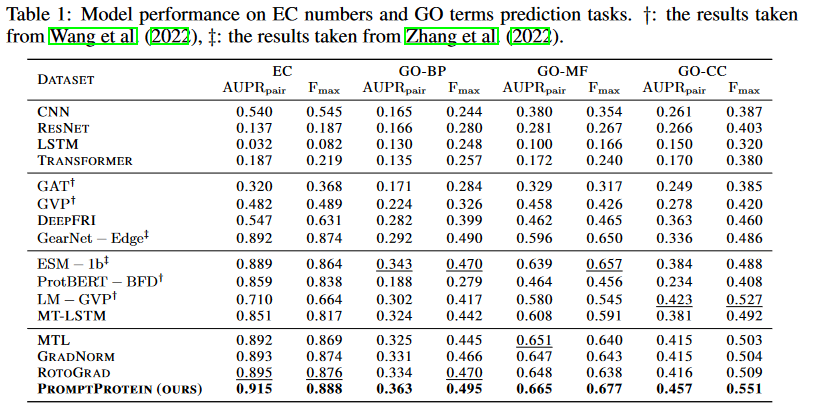
\includegraphics[width=0.9\linewidth]{figures/MPH-tab1.png}
  \end{figure}

\end{frame}



\begin{frame}{Multi-level Protein Structure Pre-training via Prompt Learning}
  \textbf{Experiments}

  \begin{itemize}
  \item downstream tasks: Protein Engineering Tasks
  \end{itemize}

  \begin{figure}[!h]
    \centering
    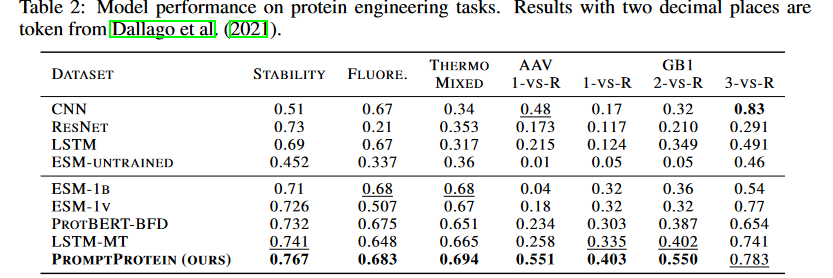
\includegraphics[width=0.9\linewidth]{figures/MPH-tab2.png}
  \end{figure}

\end{frame}




\section{Idea}
\begin{frame}
    \frametitle{Table of Contents}
    \tableofcontents[currentsection]
\end{frame}



\begin{frame}{Prompt Tuning}
  \textbf{The motivation of Prompt Tuning in language model}
  \begin{itemize}
    \item Too expensive to full fine-tune the model.  
    \item Training on insuffcient data may cause catastrophic forget.  
  \end{itemize}
\end{frame}


\begin{frame}{Prompt Tuning}
  \textbf{When model is not large enough or the downstream data are sufficient, how to achieve a compareable result based on prompt learning?}
  \begin{itemize}
    \item Visual Prompt Tuning.  
    % \item Training on insuffcient data may cause catastrophic forget.  
  \end{itemize}

  \begin{figure}[!h]
    \centering
    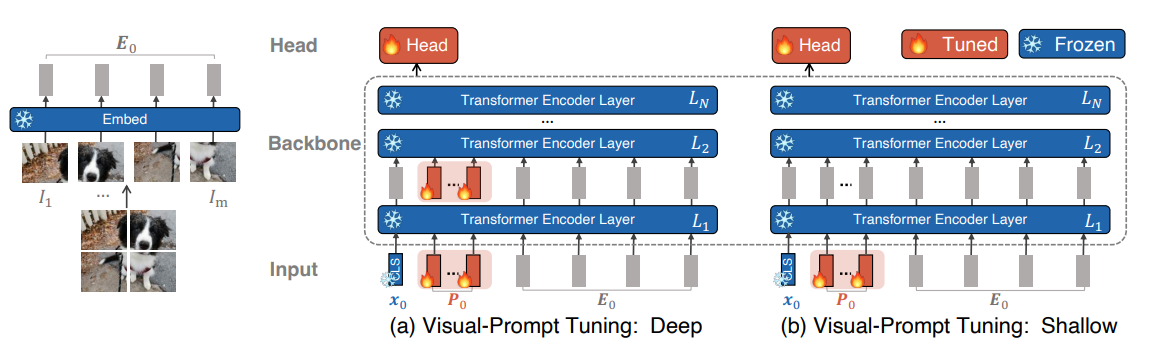
\includegraphics[width=1\linewidth]{figures/VPT-fig3.png}
  \end{figure}
\end{frame}

\begin{frame}{Prompt Tuning}
  \textbf{When model is not large enough or the downstream data are sufficient, how to achieve a compareable result based on prompt learning?}
  \begin{itemize}
    \item Visual Prompt Tuning.  
    % \item Training on insuffcient data may cause catastrophic forget.  
  \end{itemize}

  \begin{figure}[!h]
    \centering
    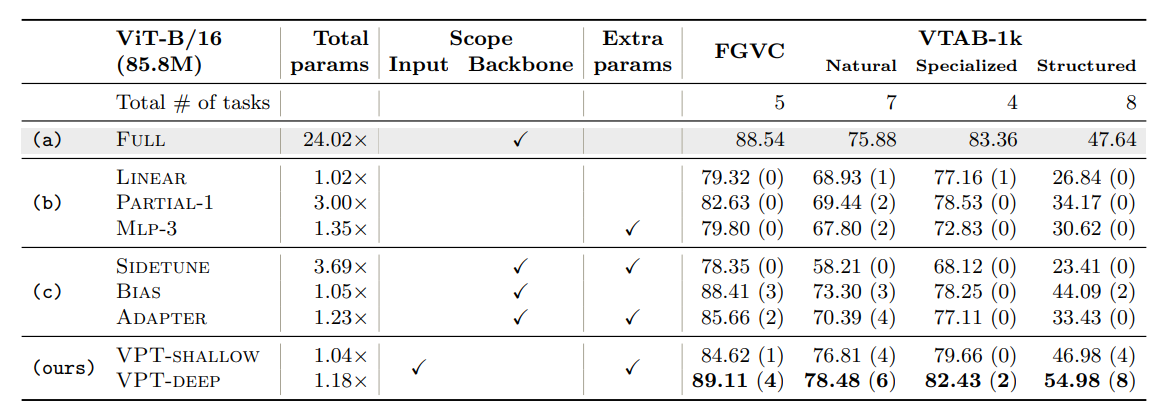
\includegraphics[width=1\linewidth]{figures/VPT-tab1.png}
  \end{figure}
\end{frame}

\begin{frame}{Prompt Tuning}
  \textbf{When model is not large enough or the downstream data are sufficient, how to achieve a compareable result based on prompt learning?}
  \begin{itemize}
    \item Few-Shot Learning(CoOp).  
    % \item Training on insuffcient data may cause catastrophic forget.  
  \end{itemize}

  \begin{figure}[!h]
    \centering
    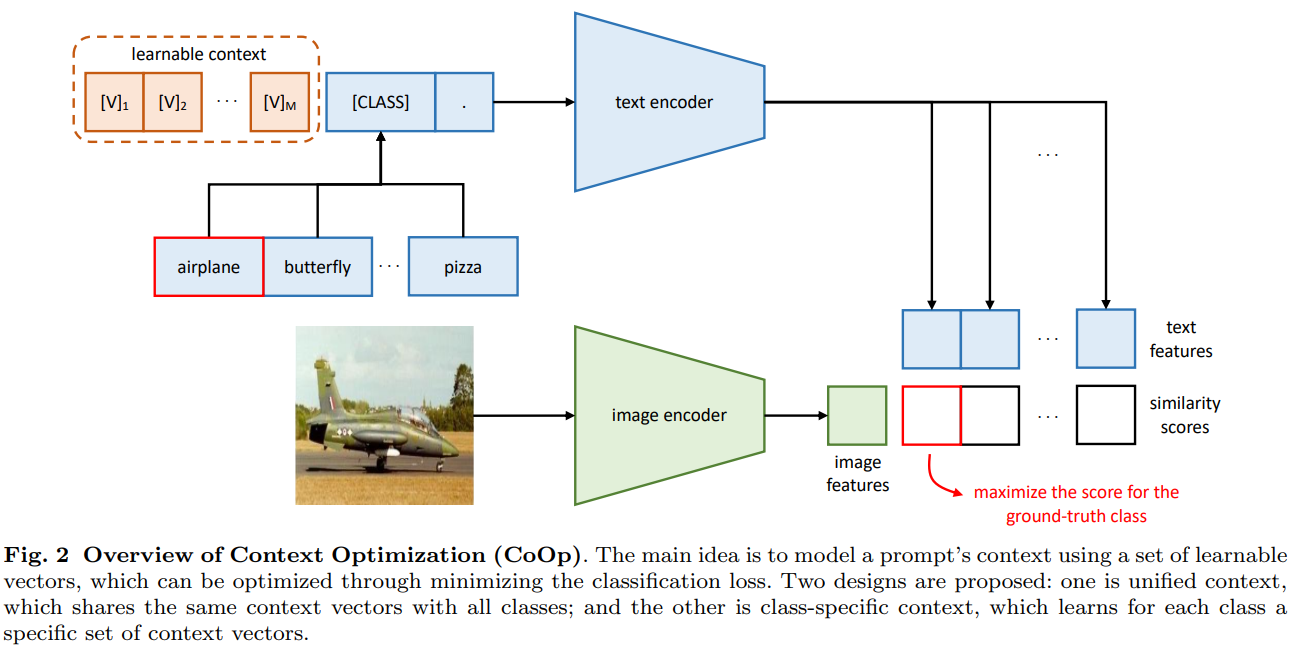
\includegraphics[width=1\linewidth]{figures/CoOp-fig2.png}
  \end{figure}
\end{frame}

\begin{frame}{Prompt Tuning}
  \textbf{When model is not large enough or the downstream data are sufficient, how to achieve a compareable result based on prompt learning?}
  \begin{itemize}
    \item Few-Shot Learning(CoOp).  
    % \item Training on insuffcient data may cause catastrophic forget.  
  \end{itemize}

  \begin{figure}[!h]
    \centering
    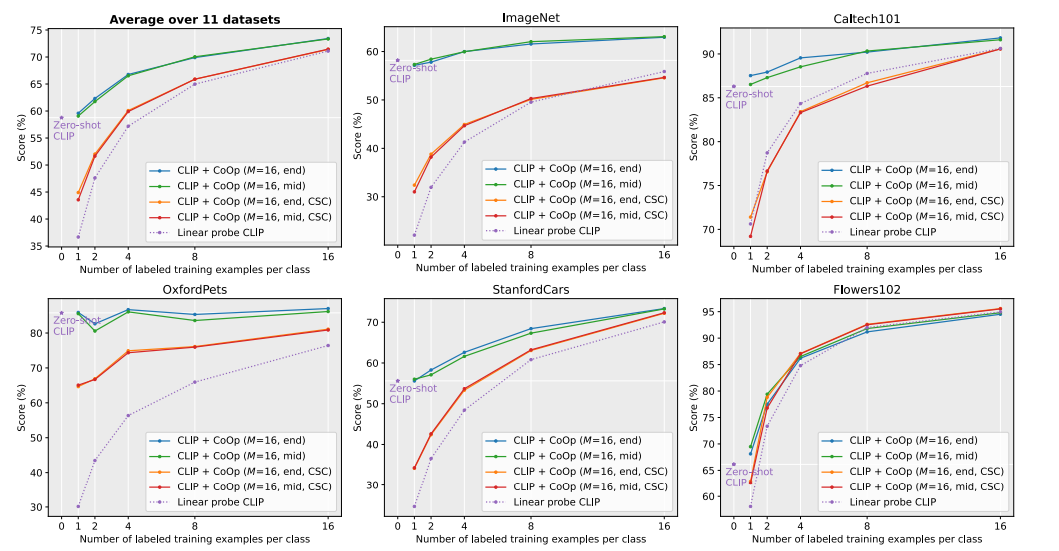
\includegraphics[width=0.9\linewidth]{figures/CoOp-fig3.png}
  \end{figure}
\end{frame}

\end{document}